\documentclass[12pt, titlepage]{article}

\usepackage{fullpage}
\usepackage[round]{natbib}
\usepackage{multirow}
\usepackage{booktabs}
\usepackage{tabularx}
\usepackage{graphicx}
\usepackage{float}
\usepackage{hyperref}
\usepackage{soul}
\usepackage{longtable}

\hypersetup{
    colorlinks,
    citecolor=blue,
    filecolor=black,
    linkcolor=red,
    urlcolor=blue
}

%% Comments

\usepackage{color}

\newif\ifcomments\commentstrue %displays comments
%\newif\ifcomments\commentsfalse %so that comments do not display

\ifcomments
\newcommand{\authornote}[3]{\textcolor{#1}{[#3 ---#2]}}
\newcommand{\todo}[1]{\textcolor{red}{[TODO: #1]}}
\else
\newcommand{\authornote}[3]{}
\newcommand{\todo}[1]{}
\fi

\newcommand{\wss}[1]{\authornote{blue}{SS}{#1}} 
\newcommand{\plt}[1]{\authornote{magenta}{TPLT}{#1}} %For explanation of the template
\newcommand{\an}[1]{\authornote{cyan}{Author}{#1}}

%% Common Parts

\newcommand{\progname}{McMaster Engineering Society Custom Financial
Expense Reporting Platform} % PUT YOUR PROGRAM NAME HERE
\newcommand{\authname}{Team \#12, Reimbursement Rangers
\\ Adam Podolak
\\ Evan Sturmey
\\ Christian Petricca
\\ Austin Bennett
\\ Jacob Kish} % AUTHOR NAMES                  

\usepackage{hyperref}
    \hypersetup{colorlinks=true, linkcolor=blue, citecolor=blue, filecolor=blue,
                urlcolor=blue, unicode=false}
    \urlstyle{same}
                                


\newcounter{acnum}
\newcommand{\actheacnum}{AC\theacnum}
\newcommand{\acref}[1]{AC\ref{#1}}

\newcounter{ucnum}
\newcommand{\uctheucnum}{UC\theucnum}
\newcommand{\uref}[1]{UC\ref{#1}}

\newcounter{mnum}
\newcommand{\mthemnum}{M\themnum}
\newcommand{\mref}[1]{M\ref{#1}}
%
\begin{document}

\title{Module Guide for \progname{}} 
\author{\authname}
\date{\today}

\maketitle

\pagenumbering{roman}

\section{Revision History}

\begin{tabularx}{\textwidth}{p{3cm}p{2cm}X}
\toprule {\bf Date} & {\bf Version} & {\bf Notes}\\
\midrule
1/17/2025 & 0 & All sections\\
3/24/2025 & 1 & Updated Authentication, see commit: \href{https://github.com/ausbennett/mes-finance-platform/commit/4cef88de4d7c2a664fa8e2395804251c0a6baeb4}{4cef88d}\\
4/4/2025 & 1 & Updated User Dashboard Module, see commit: \href{https://github.com/ausbennett/mes-finance-platform/commit/a23d43b84b1426d0f6a8d13d3120043a0d8c54b3}{a23d43b}\\
4/4/2025 & 1 & Improvements to Software decision module section, see commit: \href{https://github.com/ausbennett/mes-finance-platform/commit/d28cc2c30433566afcd2b0621950a5832a6cc40e}{d28cc2c}\\
4/4/2025 & 1 & Improved traceability tables with descriptions for what each module does, see commit: \href{https://github.com/ausbennett/mes-finance-platform/commit/6ba09e4a79e3f6a3cf5ef14b3514668898f55438}{6ba09e4}\\
4/4/2025 & 1 & Adding implementation specifics into 7.3, see commit: \href{https://github.com/ausbennett/mes-finance-platform/commit/fac3aa1adfd32881adc95c603df28100f891b46a}{fac3aa1}\\
4/4/2025 & 1 & Improving readability in anticipated changes section, see commit: \href{https://github.com/ausbennett/mes-finance-platform/commit/0cc3ad45ad4c4781cc4ed82fac16693b40476860}{0cc3ad4}\\
4/4/2025 & 1 & Adding description to use hierarchy diagram to improve readability, see commit: \href{https://github.com/ausbennett/mes-finance-platform/commit/6d4b62aad45c5ffa42d97915b147907c9c27d511}{6d4b62a}\\
\bottomrule
\end{tabularx}

\newpage

\section{Reference Material}

This section records information for easy reference.

\subsection{Abbreviations and Acronyms}

\renewcommand{\arraystretch}{1.2}
\resizebox{\textwidth}{!}{%
\begin{tabular}{ll} 
  \toprule		
  \textbf{Symbol} & \textbf{Description}\\
  \midrule 
  AC & Anticipated Change\\
  DAG & Directed Acyclic Graph \\
  M & Module \\
  MG & Module Guide \\
  OS & Operating System \\
  R & Requirement\\
  SC & Scientific Computing \\
  SRS & Software Requirements Specification\\
  \texttt{\textbackslash progname} & Explanation of program name\\
  UC & Unlikely Change \\
  \bottomrule
\end{tabular}
}

\newpage

\tableofcontents

\listoftables

\listoffigures

\newpage

\pagenumbering{arabic}

\section{Introduction}

Decomposing a system into modules is a commonly accepted approach to developing
software.  A module is a work assignment for a programmer or programming
team.  We advocate a decomposition
based on the principle of information hiding.  This
principle supports design for change, because the ``secrets'' that each module
hides represent likely future changes.  Design for change is valuable in SC,
where modifications are frequent, especially during initial development as the
solution space is explored.  

Our design follows the rules layed out by, as follows:
\begin{itemize}
\item System details that are likely to change independently should be the
  secrets of separate modules.
\item Each data structure is implemented in only one module.
\item Any other program that requires information stored in a module's data
  structures must obtain it by calling access programs belonging to that module.
\end{itemize}

After completing the first stage of the design, the Software Requirements
Specification (SRS), the Module Guide (MG) is developed. The MG
specifies the modular structure of the system and is intended to allow both
designers and maintainers to easily identify the parts of the software.  The
potential readers of this document are as follows:

\begin{itemize}
\item New project members: This document can be a guide for a new project member
  to easily understand the overall structure and quickly find the
  relevant modules they are searching for.
\item Maintainers: The hierarchical structure of the module guide improves the
  maintainers' understanding when they need to make changes to the system. It is
  important for a maintainer to update the relevant sections of the document
  after changes have been made.
\item Designers: Once the module guide has been written, it can be used to
  check for consistency, feasibility, and flexibility. Designers can verify the
  system in various ways, such as consistency among modules, feasibility of the
  decomposition, and flexibility of the design.
\end{itemize}

The rest of the document is organized as follows. Section
\ref{SecChange} lists the anticipated and unlikely changes of the software
requirements. Section \ref{SecMH} summarizes the module decomposition that
was constructed according to the likely changes. Section \ref{SecConnection}
specifies the connections between the software requirements and the
modules. Section \ref{SecMD} gives a detailed description of the
modules. Section \ref{SecTM} includes two traceability matrices. One checks
the completeness of the design against the requirements provided in the SRS. The
other shows the relation between anticipated changes and the modules. Section
\ref{SecUse} describes the use relation between modules.

\section{Anticipated and Unlikely Changes} \label{SecChange}

This section lists possible changes to the system. According to the likeliness
of the change, the possible changes are classified into two
categories. Anticipated changes are listed in Section \ref{SecAchange}, and
unlikely changes are listed in Section \ref{SecUchange}.

\subsection{Anticipated Changes} \label{SecAchange}

Anticipated changes are the source of the information that is to be hidden
inside the modules. Ideally, changing one of the anticipated changes will only
require changing the one module that hides the associated decision. The approach
adapted here is called design for
change.

\begin{description}
\item[\refstepcounter{acnum} \actheacnum \label{acDataSchema}:] Changes to the database schema to meet evolving data storage needs.
\item[\refstepcounter{acnum} \actheacnum \label{acNotifications}:] Expansion of the notification system to include push notifications and SMS.
\item[\refstepcounter{acnum} \actheacnum \label{acCompliance}:] Adjustments to the ledger views for new regulatory compliance requirements impacting data handling.
\item[\refstepcounter{acnum} \actheacnum \label{acUI}:] Enhancements to the user interface for improved accessibility and user experience.
\item[\refstepcounter{acnum} \actheacnum \label{acIntegration}:] Integration with additional third-party APIs for payment processing.
\item[\refstepcounter{acnum} \actheacnum \label{acLogin}:] Security enhancements to the login process. (i.e Integrated 2FA McMaster Login )
\end{description}

\wss{Anticipated changes relate to changes that would be made in requirements,
design or implementation choices.  They are not related to changes that are made
at run-time, like the values of parameters.}

\subsection{Unlikely Changes} \label{SecUchange}

The module design should be as general as possible. However, a general system is
more complex. Sometimes this complexity is not necessary. Fixing some design
decisions at the system architecture stage can simplify the software design. If
these decision should later need to be changed, then many parts of the design
will potentially need to be modified. Hence, it is not intended that these
decisions will be changed.

\begin{description}
\item[\refstepcounter{ucnum} \uctheucnum \label{ucArchitecture}:] Major changes to the core system architecture, such as switching from cloud to on-premises infrastructure.
\item[\refstepcounter{ucnum} \uctheucnum \label{ucLanguages}:] Transitioning from the existing programming language stack to a completely different stack.
\item[\refstepcounter{ucnum} \uctheucnum \label{ucCoreModules}:] Removal of essential core modules such as authentication or role-based access control.
\item[\refstepcounter{ucnum} \uctheucnum \label{ucProtocols}:] Fundamental changes in the communication protocols, such as moving from REST to an entirely different protocol.
\end{description}

\section{Module Hierarchy} \label{SecMH}

This section provides an overview of the module design. Modules are summarized
in a hierarchy decomposed by secrets in Table \ref{TblMH}. The modules listed
below, which are leaves in the hierarchy tree, are the modules that will
actually be implemented.

\begin{description}
\item [\refstepcounter{mnum} \mthemnum \label{mHH}:] Hardware-Hiding Module
\item [\refstepcounter{mnum} \mthemnum \label{mBH1}:] Account Management Module
\item [\refstepcounter{mnum} \mthemnum \label{mBH2}:] Requests Module
\item [\refstepcounter{mnum} \mthemnum \label{mBH3}:] Notification Module
\item [\refstepcounter{mnum} \mthemnum \label{mBH4}:] User Dashboard Module
\item [\refstepcounter{mnum} \mthemnum \label{mBH5}:] \st{Authentication Module}
\item [\refstepcounter{mnum} \mthemnum \label{mBH6}:] Email Module
\item [\refstepcounter{mnum} \mthemnum \label{mBH7}:] Account Management Controller Module
\item [\refstepcounter{mnum} \mthemnum \label{mBH8}:] Requests Controller Module
\item [\refstepcounter{mnum} \mthemnum \label{mSD1}:] Clubs Database
\item [\refstepcounter{mnum} \mthemnum \label{mSD2}:] Users Database
\item [\refstepcounter{mnum} \mthemnum \label{mSD3}:] Requests Database
\item [\refstepcounter{mnum} \mthemnum \label{mSD4}:] Graphical User Interface
\end{description}


\begin{table}[h!]
\centering
\begin{tabular}{p{0.3\textwidth} p{0.6\textwidth}}
\toprule
\textbf{Level 1} & \textbf{Level 2}\\
\midrule

{Hardware-Hiding Module} & ~ \\
\midrule

\multirow{7}{0.3\textwidth}{Behaviour-Hiding Module} 
& Account Management Module\\
& Requests Module\\
& Notification Module\\
& User Dashboard Module\\
& Authentication Module\\
& Email Module\\
& Account Management Controller Module\\
& Requests Controller Module\\
\midrule

\multirow{3}{0.3\textwidth}{Software Decision Module} 
& Clubs Database\\
& Users Database\\
& Requests Database\\
& Graphical User Interface\\
\bottomrule

\end{tabular}
\caption{Module Hierarchy}
\label{TblMH}
\end{table}

\section{Connection Between Requirements and Design} \label{SecConnection}

The design of the system is intended to satisfy the requirements developed in
the SRS. In this stage, the system is decomposed into modules. The connection
between requirements and modules is listed in Table~\ref{TblRT}.

\wss{The intention of this section is to document decisions that are made
  ``between'' the requirements and the design.  To satisfy some requirements,
  design decisions need to be made.  Rather than make these decisions implicit,
  they are explicitly recorded here.  For instance, if a program has security
  requirements, a specific design decision may be made to satisfy those
  requirements with a password.}

\section{Module Decomposition} \label{SecMD}

Modules are decomposed according to the principle of ``information hiding''
proposed by \citet{ParnasEtAl1984}. The \emph{Secrets} field in a module
decomposition is a brief statement of the design decision hidden by the
module. The \emph{Services} field specifies \emph{what} the module will do
without documenting \emph{how} to do it. For each module, a suggestion for the
implementing software is given under the \emph{Implemented By} title. If the
entry is \emph{OS}, this means that the module is provided by the operating
system or by standard programming language libraries.  \emph{\progname{}} means the
module will be implemented by the \progname{} software.

Only the leaf modules in the hierarchy have to be implemented. If a dash
(\emph{--}) is shown, this means that the module is not a leaf and will not have
to be implemented.

\subsection{Hardware Hiding Modules (\mref{mHH})}

\begin{description}
\item[Secrets:]The data structure and algorithm used to implement the virtual
  hardware.
\item[Services:]Serves as a virtual hardware used by the rest of the
  system. This module provides the interface between the hardware and the
  software. So, the system can use it to display outputs or to accept inputs.
\item[Implemented By:] OS
\end{description}

\subsection{Behaviour-Hiding Module}

\begin{description}
\item[Secrets:]The contents of the required behaviours.
\item[Services:]Includes programs that provide externally visible behaviour of
  the system as specified in the software requirements specification (SRS)
  documents. This module serves as a communication layer between the
  hardware-hiding module and the software decision module. The programs in this
  module will need to change if there are changes in the SRS.
\item[Implemented By:] --
\end{description}

\subsubsection{Account Management Module (\mref{mBH1})}

\begin{description}
\item[Secrets:] User account details, including personal information, access levels, and account statuses.
\item[Services:] Provides functionality for creating, updating, and deleting user accounts. It manages user roles and permissions, ensuring that appropriate access is granted to each user based on their role within the system. This module ensures secure storage of account information and integrates with the authentication module for login and identity verification purposes.
\item[Implemented By:] Account Management Controller
\item[Type of Module:] Abstract Data Type
\end{description}

\subsubsection{Requests Module (\mref{mBH2})}

\begin{description}
\item[Secrets:] Internal data structure of requests, including status, history, and associated user transaction information.
\item[Services:] Manages the creation, tracking, and approval of reimbursement requests. This module handles the submission of new requests by users, updates the status of existing requests, and reconcilies transactions with external plaid API for auditing purposes. It communicates with the notification module to inform users about the progress of their requests.
\item[Implemented By:] Requests Controller
\item[Type of Module:] Abstract Data Type
\end{description}

\subsubsection{Notification Module (\mref{mBH3})}

\begin{description}
\item[Secrets:] Notification content, delivery methods, and scheduling information.
\item[Services:] Sends notifications to users regarding updates to their reimbursement requests, account changes, and other system events. It supports email. The module ensures that notifications are timely.
\item[Implemented By:] Emailer API
\item[Type of Module:] Abstract Data Type
\end{description}

\subsubsection{User Dashboard Module (\mref{mBH4})}

\begin{description}
\item{Secrets:} Defines the organization and structure of displayed data, including summaries and real-time updates.

\item{Services:} Delivers a user-friendly interface showing the current status of reimbursement requests, notifications, and account information. It updates dynamically based on user interactions and backend data changes. Real-time updates are handled through periodic polling, ensuring timely reflection of state changes while maintaining performance efficiency. The module integrates with the requests and account management modules to provide a comprehensive, up-to-date user experience.

\item[Implemented By:] MRM
\item[Type of Module:] Abstract Data Type
\end{description}

\subsubsection{Authentication Module (\mref{mBH5})}
\textit{This was deemed out of scope. Authentication will be done through integrating with MES' existing authentication process.}
\begin{description}
\item[Secrets:] \st{Validation processes, and session management details.}
\item[Services:] \st{Handles user login, logout, and session management. It ensures secure authentication using encrypted credentials. The module integrates with the account management module to verify user identities and enforce access control.}


\item[Implemented By:] \st{MRM}
\item[Type of Module:] \st{Abstract Data Type} 
\end{description}

\subsubsection{Emailer API (\mref{mBH6})}

\begin{description}
\item[Secrets:] Email templates, SMTP server credentials.
\item[Services:] Provides an interface for sending emails to users. It handles notification delivery, and verification communications, and ensures successful delivery through integration with external SMTP services. The module is used by the notification module to send email-based alerts to users.
\item[Implemented By:] TBD
\item[Type of Module:] Abstract Data Type
\end{description}

\subsubsection{Account Management Controller (\mref{mBH7})}

\begin{description}
\item[Secrets:] The flow of control for account operations and error handling mechanisms.
\item[Services:] Acts as a controller for the account management module. It receives requests from the user dashboard and other modules, processes them, and invokes appropriate functions within the account management module. It ensures consistency and error handling in account-related operations.
\item[Implemented By:] MRM
\item[Type of Module:] Abstract Data Type
\end{description}

\subsubsection{Requests Controller (\mref{mBH8})}

\begin{description}
\item[Secrets:] The flow of control for request operations and error handling mechanisms.
\item[Services:] Acts as a controller for the requests module. It handles user inputs for creating and managing requests, processes these inputs, and invokes the necessary functions within the requests module. The controller ensures that all requests are valid and consistent with the system’s requirements.
\item[Implemented By:] MRM
\item[Type of Module:] Abstract Data Type
\end{description}

\subsection{Software Decision Module}

\begin{description}
\item[Secrets:] The design decision based on mathematical theorems, physical
  facts, or programming considerations. The secrets of this module are
  \emph{not} described in the SRS.
\item[Services:] This module encompasses the system's data storage components that do not provide direct interaction with the user but support core functionalities. The databases are responsible for reliable transaction handling and efficient data querying. They expose methods to relevant controllers and modules to facilitate logic. These modules are designed with scalability in mind, including support for integration with third-party APIs (e.g., payment processors) and extendable schema models for anticipated data format changes. 
  % Changes in these modules are more likely to be motivated by a desire to
  % improve performance than by externally imposed changes.
\item[Implemented By:] MongoDB
\end{description}

\subsubsection{Clubs Database (\mref{mSD1})}

\begin{description}
\item[Secrets:] The structure and format of the database storing information about McMaster University clubs, including club names, member rosters, and financial data.
\item[Services:] Provides methods to store, retrieve, and update club-related data, ensuring data integrity and quick access. It supports queries for club membership, financial histories, and active/inactive statuses, which are used by other modules to process reimbursement requests.
\item[Implemented By:] MongoDB
\item[Type of Module:] Library
\end{description}

\subsubsection{User Database (\mref{mSD2})}

\begin{description}
\item[Secrets:] The structure and format of the database storing user account details, including personal information, roles, and activity logs.
\item[Services:] Stores user registration data, access roles, and status fields. Interfaces with the Authentication Module to verify user identity and with the Account Management Module to fetch/update user details. 

purposes.
\item[Implemented By:] MongoDB
\item[Type of Module:] Library
\end{description}

\subsubsection{Requests Database (\mref{mSD3})}

\begin{description}
\item[Secrets:] The structure and format of the database containing reimbursement request records, including statuses, timestamps, and related documents.
\item[Services:] Manages creation and updates of reimbursement/payment requests from the Requests Module. Supports historical tracking via logs and timestamps. Ensures transaction integrity when updates are made through the Requests Controller. Interacts with third-party APIs (e.g., Plaid or payment systems) to log transaction results.
\item[Implemented By:] MongoDB
\item[Type of Module:] Library
\end{description}

\subsubsection{Graphical User Interface (\mref{mSD4})}

\begin{description}
\item[Secrets:] The structure and layout of user interaction elements, including buttons, forms, and visual themes. It also contains methods to style and manage user inputs efficiently.
\item[Services:] Builds a visual interface for users to interact with the platform. Handles user input events (e.g., button clicks, form submissions) and sends commands to the appropriate modules. Provides error handling for invalid inputs and visual feedback.
\item[Implemented By:] React
\item[Type of Module:] Library
\end{description}


\section{Traceability Matrix} \label{SecTM}

This section shows two traceability matrices: between the modules and the
requirements and between the modules and the anticipated changes. Note: hyperlinks to requirements in the SRS will be added in a later version of this document.

% the table should use mref, the requirements should be named, use something
% like fref
\begin{longtable}{p{0.15\textwidth} p{0.45\textwidth} p{0.3\textwidth}}
\caption{Trace Between Requirements and Modules with Notes} \\
\toprule
\textbf{Req.} & \textbf{Modules} & \textbf{Notes} \\
\midrule
\endfirsthead

\multicolumn{3}{c}%
{{\bfseries \tablename\ \thetable{} -- continued from previous page}} \\
\toprule
\textbf{Req.} & \textbf{Modules} & \textbf{Notes} \\
\midrule
\endhead

\bottomrule
\endfoot

\href{../../SRS/SRS.pdf#FROneOne}{ FR1.1 } & \mref{mBH2}, \mref{mBH4}, \mref{mBH8}, \mref{mSD1}, \mref{mSD2}, \mref{mSD3}, \mref{mSD4} & Request handling, UI display, data persistence \\
\href{../../SRS/SRS.pdf#FROneTwo}{ FR1.2 } & \mref{mBH2}, \mref{mBH4}, \mref{mBH8}, \mref{mSD1}, \mref{mSD2}, \mref{mSD3}, \mref{mSD4} & Edit flow across controller, DBs, and UI \\
\href{../../SRS/SRS.pdf#FROneThree}{ FR1.3 } & \mref{mBH2}, \mref{mBH4}, \mref{mBH8}, \mref{mSD1}, \mref{mSD2}, \mref{mSD3}, \mref{mSD4} & Full request lifecycle coverage \\
\href{../../SRS/SRS.pdf#FROneFour}{ FR1.4 } & \mref{mBH2}, \mref{mBH4}, \mref{mBH8}, \mref{mSD1}, \mref{mSD2}, \mref{mSD3}, \mref{mSD4} & Same modules involved in view/edit flow \\
\href{../../SRS/SRS.pdf#FROneFive}{ FR1.5 } & \mref{mBH3}, \mref{mBH6} & Email delivery and template management \\
\href{../../SRS/SRS.pdf#FROneSix}{ FR1.6 } & \mref{mSD3} & Request status tracking \\
\href{../../SRS/SRS.pdf#FROneSeven}{ FR1.7 } & \mref{mBH5} & Handles authentication \\
\href{../../SRS/SRS.pdf#FROneEight}{ FR1.8 } & \mref{mBH4}, \mref{mBH2}, \mref{mBH8}, \mref{mSD4} & UI (M13), request DB (M12), controller (M9), and logic (M3) \\
\href{../../SRS/SRS.pdf#FROneNine}{ FR1.9 } & \mref{mSD3} & Tracks updates in request database \\
\href{../../SRS/SRS.pdf#FRThreeOne}{ FR3.1 } & \mref{mSD1}, \mref{mSD2} & User/club info persistence \\
\href{../../SRS/SRS.pdf#FRThreeTwo}{ FR3.2 } & \mref{mBH5} & Authentication via existing MES system \\
\href{../../SRS/SRS.pdf#FRThreeThree}{ FR3.3 } & \mref{mBH1}, \mref{mBH7} & Account management and controller logic \\
\href{../../SRS/SRS.pdf#APROne}{ APR1 } & \mref{mSD4} & Responsive frontend design \\
\href{../../SRS/SRS.pdf#APRTwo}{ APR2 } & \mref{mSD4} & UI enhancement handling \\
\href{../../SRS/SRS.pdf#STYROne}{ STYR1 } & \mref{mSD4} & GUI styling for themes \\
\href{../../SRS/SRS.pdf#STYRTwo}{ STYR2 } & \mref{mSD4} & Accessibility theming \\
\href{../../SRS/SRS.pdf#EUROne}{ EUR1 } & \mref{mSD4} & UI structure \\
\href{../../SRS/SRS.pdf#EURTwo}{ EUR2 } & \mref{mSD4} & Form design layout \\
\href{../../SRS/SRS.pdf#EurThree}{ EUR3 } & \mref{mSD4} & Interactive elements \\
\href{../../SRS/SRS.pdf#PIROne}{ PIR1 } & \mref{mBH1}, \mref{mBH7} & Account roles and permissions \\
\href{../../SRS/SRS.pdf#PIRTwo}{ PIR2 } & \mref{mBH1}, \mref{mBH7} & Role editing logic \\
\href{../../SRS/SRS.pdf#UAPROne}{ UAPR1 } & \mref{mSD4} & Visual layout engine \\
\href{../../SRS/SRS.pdf#ACSROne}{ ACSR1 } & \mref{mSD4} & GUI component arrangement \\
\href{../../SRS/SRS.pdf#ACSRTwo}{ ACSR2 } & \mref{mSD4} & Frontend component styling \\
\href{../../SRS/SRS.pdf#SPLROne}{ SPLR1 } & \mref{mBH2}, \mref{mBH8}, \mref{mSD1}, \mref{mSD2}, \mref{mSD3} & Club/user/request logic coordination \\
\href{../../SRS/SRS.pdf#SPLRTwo}{ SPLR2 } & \mref{mBH2}, \mref{mBH8}, \mref{mSD1}, \mref{mSD2}, \mref{mSD3} & Multi-module reconciliation \\
\href{../../SRS/SRS.pdf#SPLRThree}{ SPLR3 } & \mref{mBH2}, \mref{mBH8}, \mref{mSD1}, \mref{mSD2}, \mref{mSD3} & Data integrity during request flow \\
\href{../../SRS/SRS.pdf#SFCROne}{ SFCR1 } & \mref{mSD2}, \mref{mSD3} & DB integrity and cross-link validation \\
\href{../../SRS/SRS.pdf#SFCRTwo}{ SFCR2 } & \mref{mBH5} & Authentication flow security \\
\href{../../SRS/SRS.pdf#POAROne}{ POAR1 } & \mref{mBH8} & Request form validation control \\

\end{longtable}

\newpage

\begin{longtable}{p{0.15\textwidth} p{0.45\textwidth} p{0.3\textwidth}}
\caption{Trace Between Additional Requirements and Modules with Notes} \\
\toprule
\textbf{Req.} & \textbf{Modules} & \textbf{Notes} \\
\midrule
\endfirsthead

\multicolumn{3}{c}%
{{\bfseries \tablename\ \thetable{} -- continued from previous page}} \\
\toprule
\textbf{Req.} & \textbf{Modules} & \textbf{Notes} \\
\midrule
\endhead

\bottomrule
\endfoot

\href{../../SRS/SRS.pdf#FROneOne}{ CPR1 } & \mref{mBH2}, \mref{mBH8} & Club/request form logic \\
\href{../../SRS/SRS.pdf#FROneOne}{ CPR2 } & \mref{mBH2}, \mref{mBH8} & Same as CPR1 with extended role validation \\
\href{../../SRS/SRS.pdf#FROneOne}{ CPR3 } & \mref{mSD1}, \mref{mSD2}, \mref{mSD3} & Core DBs for persistence of forms \\
\href{../../SRS/SRS.pdf#FROneOne}{ OR1 } & \mref{mHH} & Hardware abstraction \\
\href{../../SRS/SRS.pdf#FROneOne}{ IAR1 } & \mref{mHH} – \mref{mSD4} & Full system integration from hardware to frontend \\
\href{../../SRS/SRS.pdf#FROneOne}{ PRD1 } & \mref{mSD1}, \mref{mSD2}, \mref{mSD3} & Data model for third-party integration \\
\href{../../SRS/SRS.pdf#FROneOne}{ PRD2 } & \mref{mBH5} & Auth for secured external access \\
\href{../../SRS/SRS.pdf#FROneOne}{ PRD3 } & \mref{mSD4} & UI layer interacting with APIs \\
\href{../../SRS/SRS.pdf#FROneOne}{ PRD4 } & \mref{mHH} – \mref{mSD4} & Full stack extensibility \\
\href{../../SRS/SRS.pdf#FROneOne}{ PRD5 } & \mref{mHH} – \mref{mSD4} & Reusable across integrations \\
\href{../../SRS/SRS.pdf#FROneOne}{ PRD6 } & \mref{mHH} – \mref{mSD4} & Modular design for third-party support \\
\href{../../SRS/SRS.pdf#FROneOne}{ PRD7 } & \mref{mSD1}, \mref{mSD2}, \mref{mSD3} & Schema control for partner data \\
\href{../../SRS/SRS.pdf#FROneOne}{ RLR1 } & \mref{mHH} – \mref{mSD4} & System-wide logging and recovery \\
\href{../../SRS/SRS.pdf#FROneOne}{ MR1 } & \mref{mSD1}, \mref{mSD2}, \mref{mSD3} & DB scalability and replication \\
\href{../../SRS/SRS.pdf#FROneOne}{ MR2 } & \mref{mHH} – \mref{mSD4} & Whole-system modularity \\
\href{../../SRS/SRS.pdf#FROneOne}{ MR3 } & \mref{mHH} – \mref{mSD4} & Flexible module interconnectivity \\
\href{../../SRS/SRS.pdf#FROneOne}{ SR1 } & \mref{mHH} – \mref{mSD4} & Runtime security architecture \\
\href{../../SRS/SRS.pdf#FROneOne}{ AR1 } & \mref{mHH} – \mref{mSD4} & Architecture for extensibility \\
\href{../../SRS/SRS.pdf#FROneOne}{ SCR1 } & \mref{mBH5} & Login security \\
\href{../../SRS/SRS.pdf#FROneOne}{ SCR2 } & \mref{mBH5}, \mref{mBH1}, \mref{mBH7} & Auth, account, and controller validation \\
\href{../../SRS/SRS.pdf#FROneOne}{ SCR3 } & \mref{mBH5}, \mref{mBH3}, \mref{mBH6} & Email and auth security features \\
\href{../../SRS/SRS.pdf#FROneOne}{ SCR4 } & \mref{mBH1}, \mref{mBH7}, \mref{mBH5} & Controller role security \\
\href{../../SRS/SRS.pdf#FROneOne}{ SCR5 } & \mref{mBH1}, \mref{mBH7}, \mref{mBH5} & Consistent role-based logic \\
\href{../../SRS/SRS.pdf#FROneOne}{ SCR6 } & \mref{mBH1}, \mref{mBH7}, \mref{mBH5} & Secure module boundaries \\
\href{../../SRS/SRS.pdf#FROneOne}{ INR1 } & \mref{mBH2}, \mref{mBH8} & Request form controller logic \\
\href{../../SRS/SRS.pdf#FROneOne}{ PVR1 } & \mref{mBH1}, \mref{mBH2}, \mref{mBH3}, \mref{mBH5}, \mref{mBH6}, \mref{mBH7}, \mref{mBH8}, \mref{mSD1}, \mref{mSD2}, \mref{mSD3} & System-wide data privacy controls \\
\href{../../SRS/SRS.pdf#FROneOne}{ PVR2 } & \mref{mBH1} – \mref{mSD4} & Full system privacy enforcement \\
\href{../../SRS/SRS.pdf#FROneOne}{ ADR1 } & \mref{mBH1}, \mref{mBH2}, \mref{mBH3}, \mref{mBH5}, \mref{mBH6}, \mref{mBH7}, \mref{mBH8}, \mref{mSD1}, \mref{mSD2}, \mref{mSD3} & All data modules support change \\
\href{../../SRS/SRS.pdf#FROneOne}{ ADR2 } & \mref{mSD3} & Tracks and stores audit logs \\
\href{../../SRS/SRS.pdf#FROneOne}{ IMM1 } & \mref{mSD1}, \mref{mSD2}, \mref{mSD3} & Core DB schema updatable \\
\href{../../SRS/SRS.pdf#FROneOne}{ CLTR1 } & \mref{mSD4} & UI display of ledger totals \\
\href{../../SRS/SRS.pdf#FROneOne}{ LR1 } & \mref{mHH} – \mref{mSD4} & Logging through system layers \\
\href{../../SRS/SRS.pdf#FROneOne}{ LR2 } & \mref{mHH} – \mref{mSD4} & Recovery logic system-wide \\

\end{longtable}


\begin{table}[H]
\centering
\begin{tabular}{p{0.2\textwidth} p{0.6\textwidth}}
\toprule
\textbf{AC} & \textbf{Modules}\\
\midrule
\acref{acDataSchema} & \mref{mSD1}, \mref{mSD2}, \mref{mSD3}\\
\acref{acNotifications} & \mref{mBH3}, \mref{mBH6}\\
\acref{acCompliance} & \mref{mBH8}, \mref{mBH4}, \mref{mBH2}\\
\acref{acUI} & \mref{mSD4}\\
\acref{acIntegration} & \mref{mBH1}, \mref{mBH7}\\
\acref{acLogin} & \mref{mBH5}, \mref{mHH}\\
\bottomrule
\end{tabular}
\caption{Trace Between Anticipated Changes and Modules}
\label{TblACT}
\end{table}

\newpage

\section{Use Hierarchy Between Modules} \label{SecUse}

In this section, the uses hierarchy between modules is
provided. Of two programs A and B that A {\em uses} B if
correct execution of B may be necessary for A to complete the task described in
its specification. That is, A {\em uses} B if there exist situations in which
the correct functioning of A depends upon the availability of a correct
implementation of B.  Figure \ref{FigUH} illustrates the use relation between
the modules. It can be seen that the graph is a directed acyclic graph
(DAG). Each level of the hierarchy offers a testable and usable subset of the
system, and modules in the higher level of the hierarchy are essentially simpler because they use modules from the lower levels. In the below diagram, the different layers of the system architecture are represented. Blue indicates frontend modules, red indicates backend modules/services, and green indicates database modules/collections. In the diagram, shapes indicate the role of each component. Red rounded rectangles are APIs and controllers handling logic and communication, while red dashed rectangles show external services or internal routes. Green rounded rectangles are database modules, green rectangles are MongoDB collections, and green dashed rectangles represent the data models defining schema. The green diamond denotes file storage for uploaded assets linked to requests.

\wss{The uses relation is not a data flow diagram.  In the code there will often
be an import statement in module A when it directly uses module B.  Module B
provides the services that module A needs.  The code for module A needs to be
able to see these services (hence the import statement).  Since the uses
relation is transitive, there is a use relation without an import, but the
arrows in the diagram typically correspond to the presence of import statement.}

\wss{If module A uses module B, the arrow is directed from A to B.}

\begin{figure}[H]
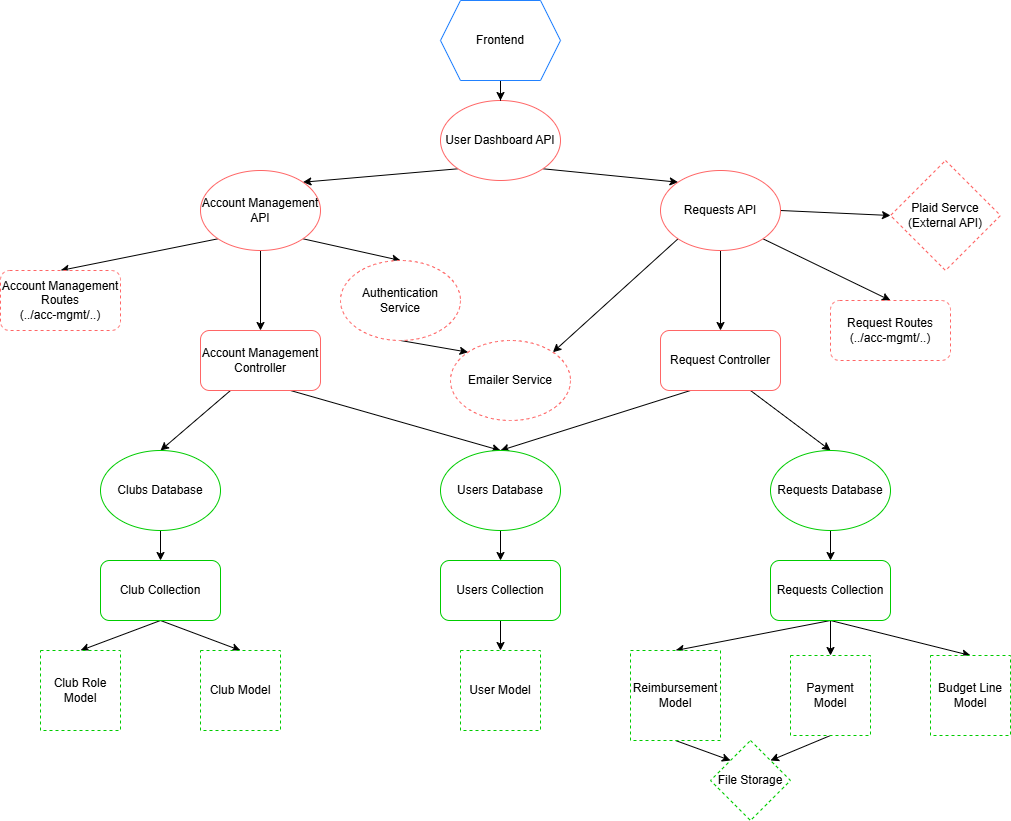
\includegraphics[width=1.1\textwidth]{imgs/UsesHierarchy.png}
\caption{Use hierarchy among modules}
\label{FigUH}
\end{figure}

%\section*{References}

\newpage

\section{User Interfaces}

Design of the user interface screens are located on \href{https://www.figma.com/design/44vRz90xLocsOkyLXjaODB/MES-Finance-Platform?node-id=0-1&t=uPGJjQawfH5iIdCy-1}{Figma}. Image references are also provided below:

\subsection{Login/Signup Page}

\includegraphics[]{imgs/LoginSignupPage.png}

\subsection{User Info Form (General Info)}
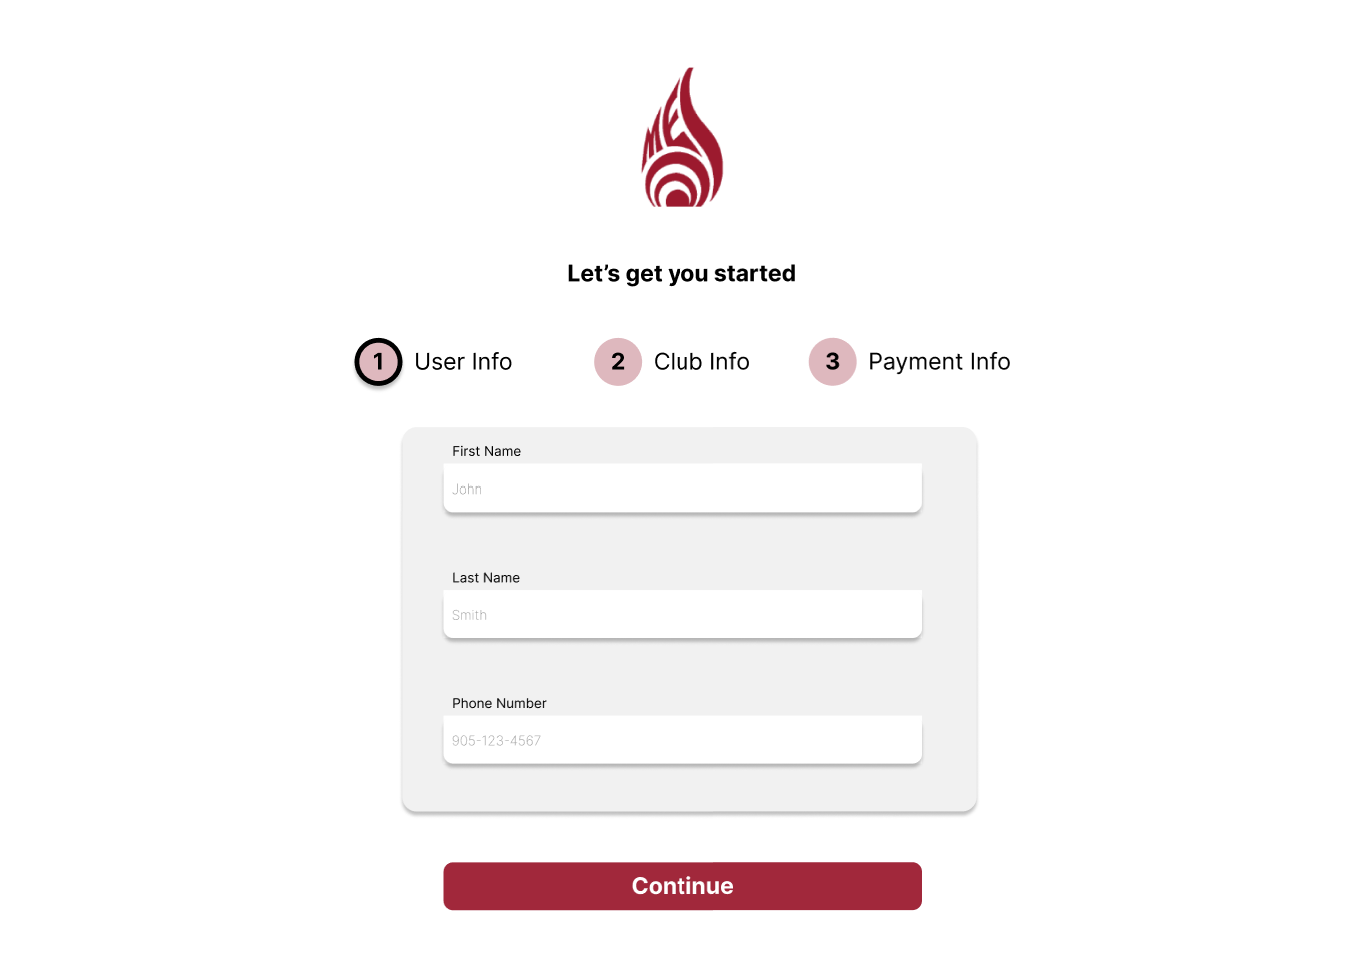
\includegraphics[]{imgs/UserInfoForm-GeneralInfo.png}

\subsection{User Info Form (Club Info)}
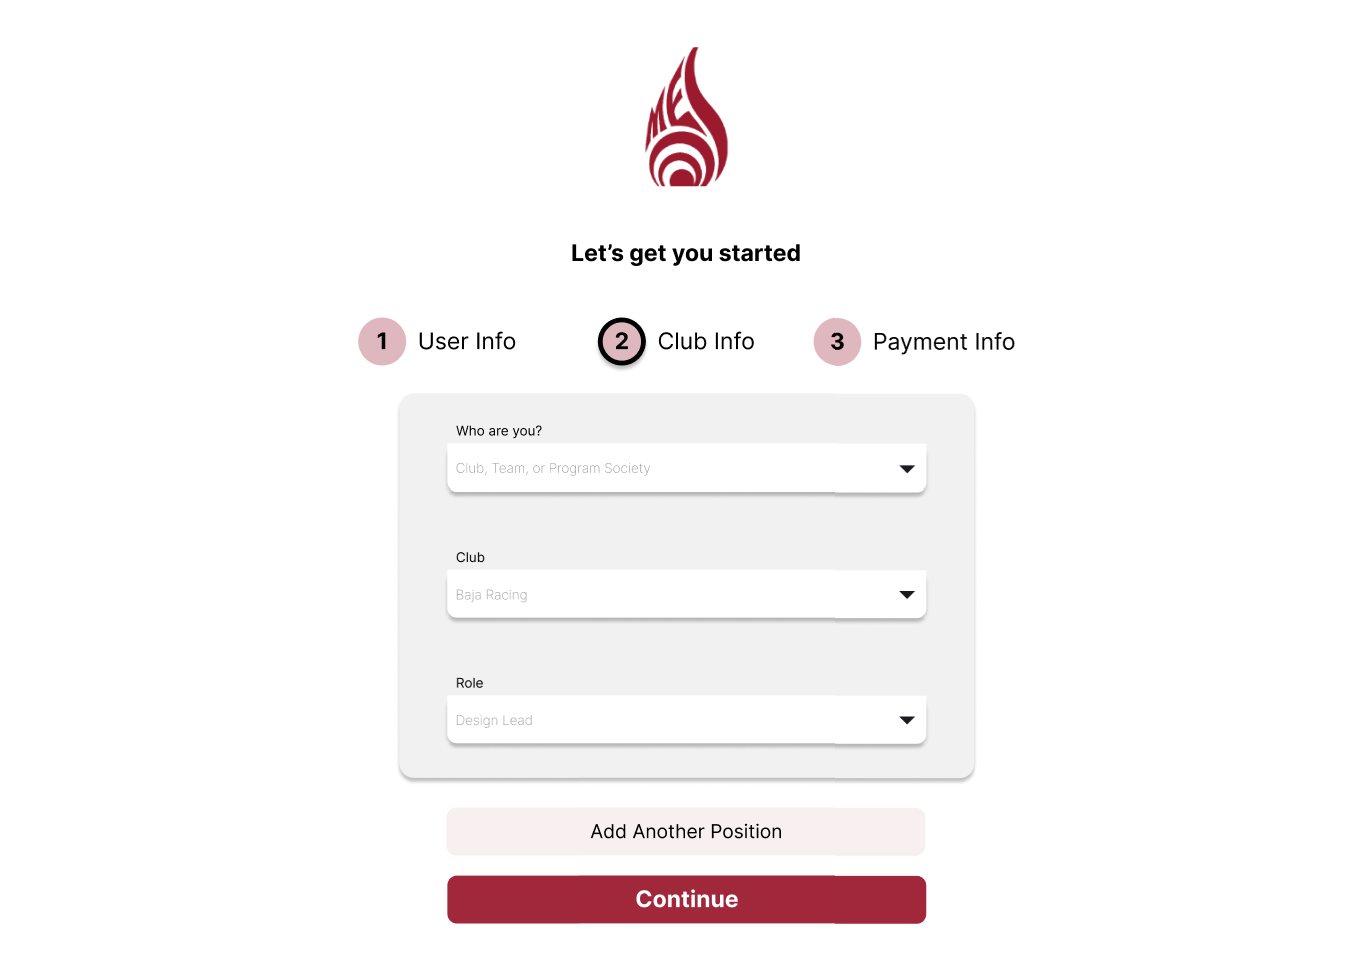
\includegraphics[]{imgs/UserInfoForm-ClubInfo.png}

\subsection{User Info Form (Payment Info)}
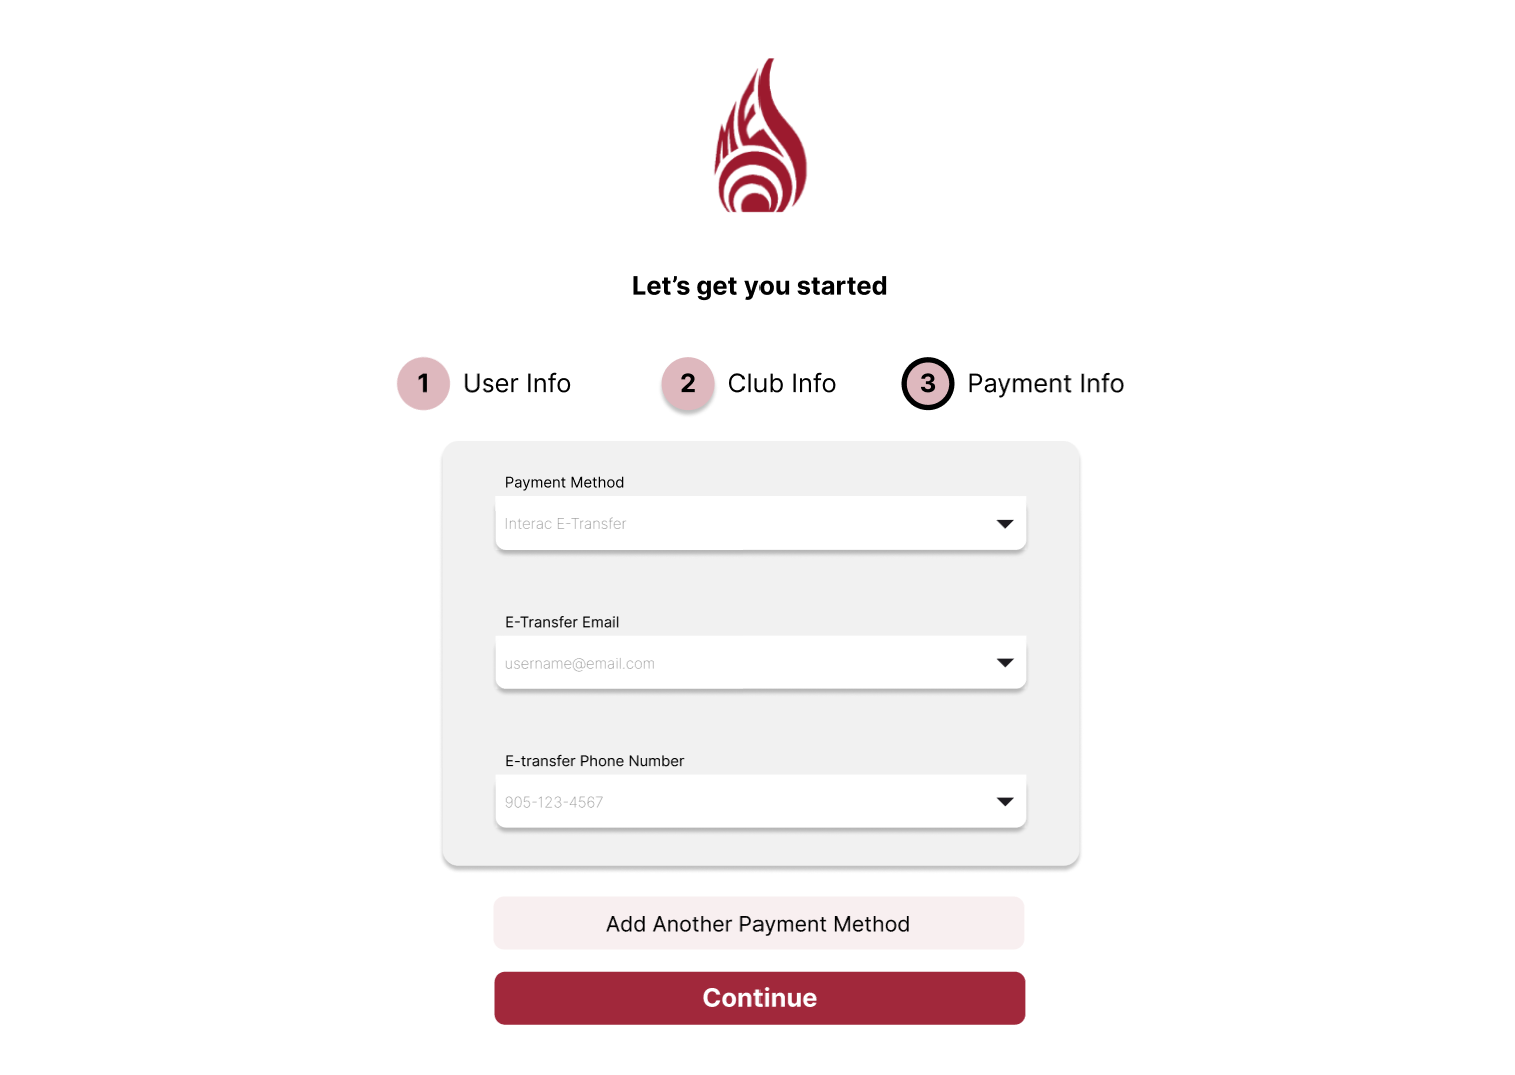
\includegraphics[]{imgs/UserInfoForm-Payment.png}

\subsection{Student Dashboard}
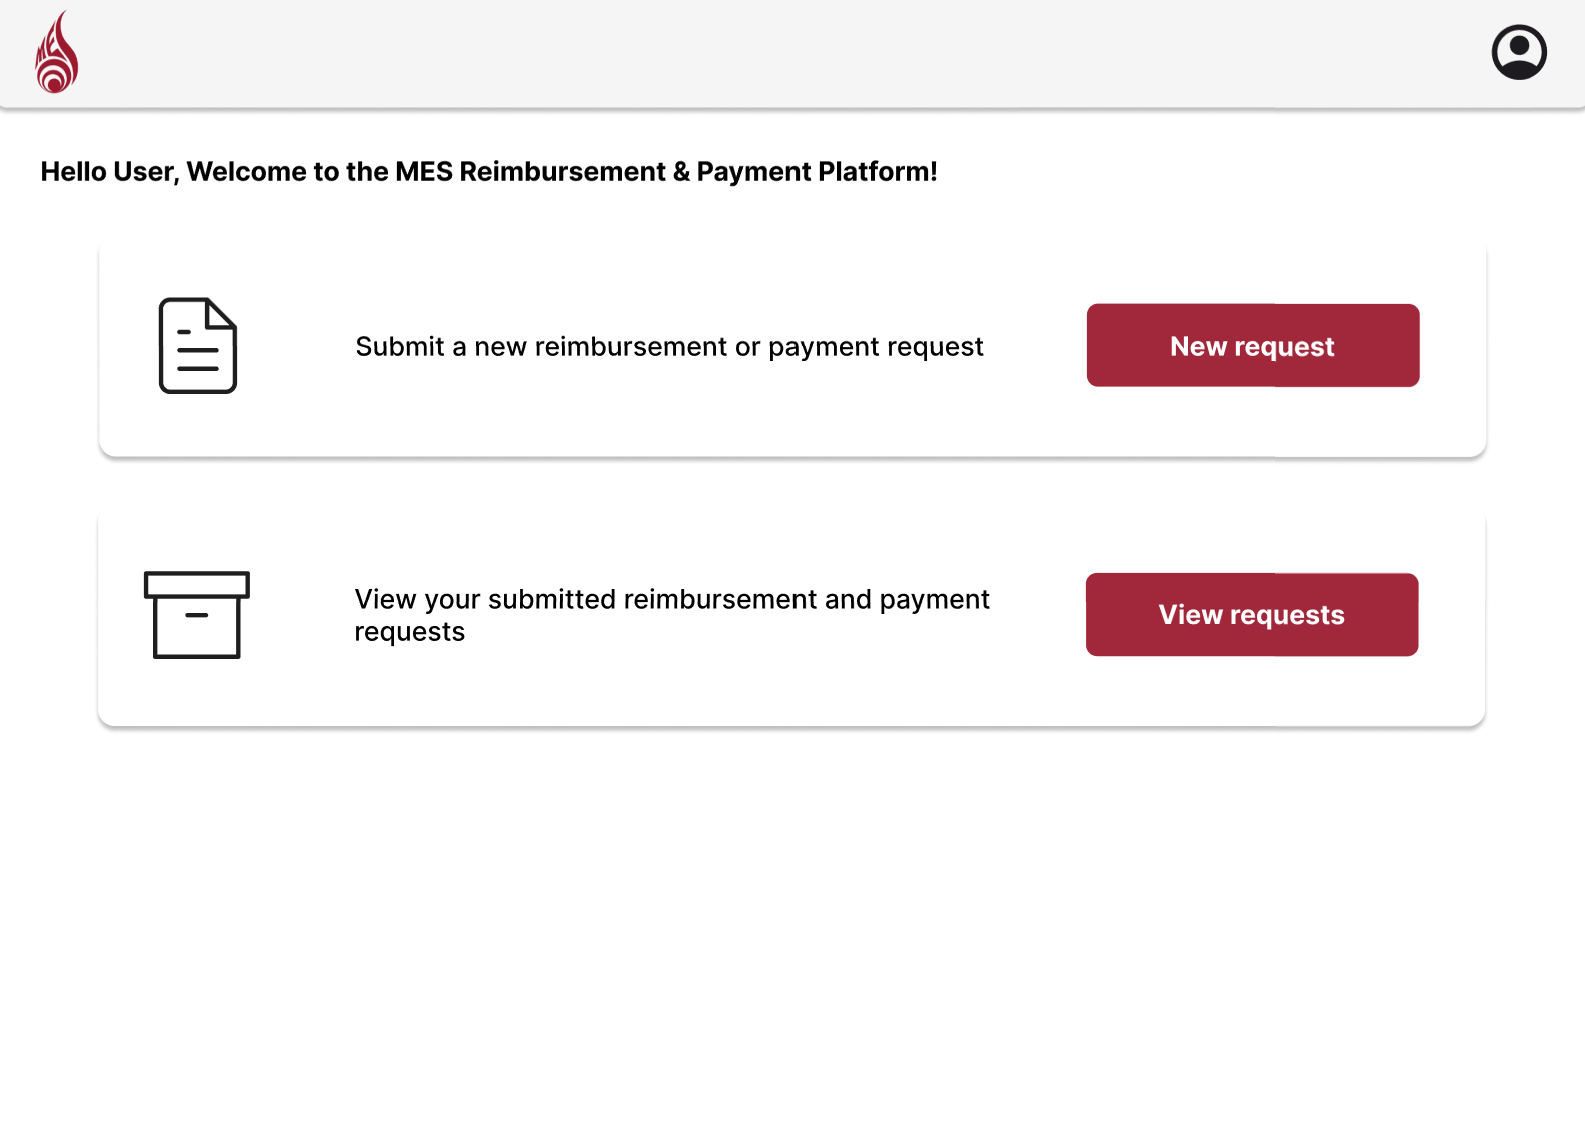
\includegraphics[]{imgs/StudentDashboard.png}

\subsection{Admin Dashboard}
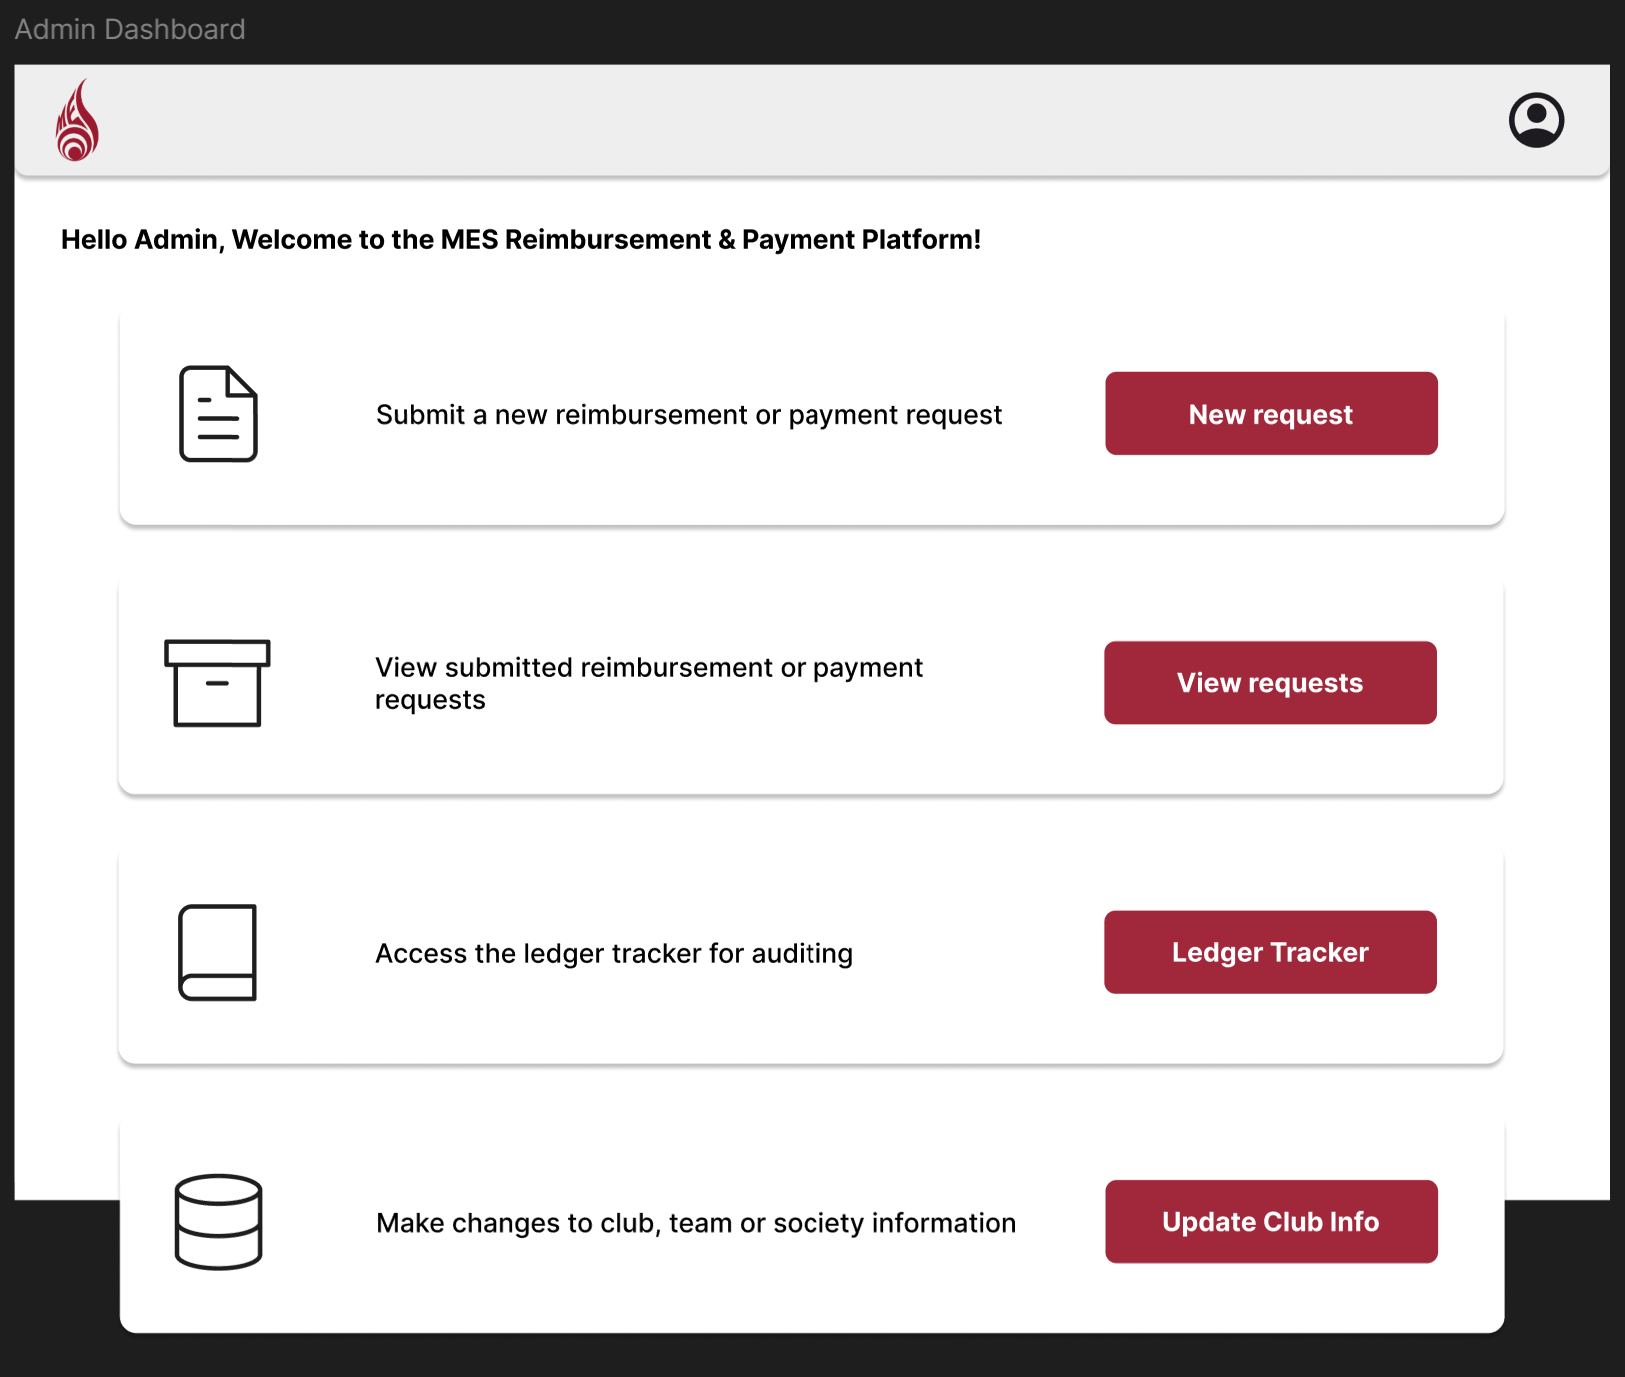
\includegraphics[]{imgs/AdminDashboard.png}

\subsection{Account Info Page}
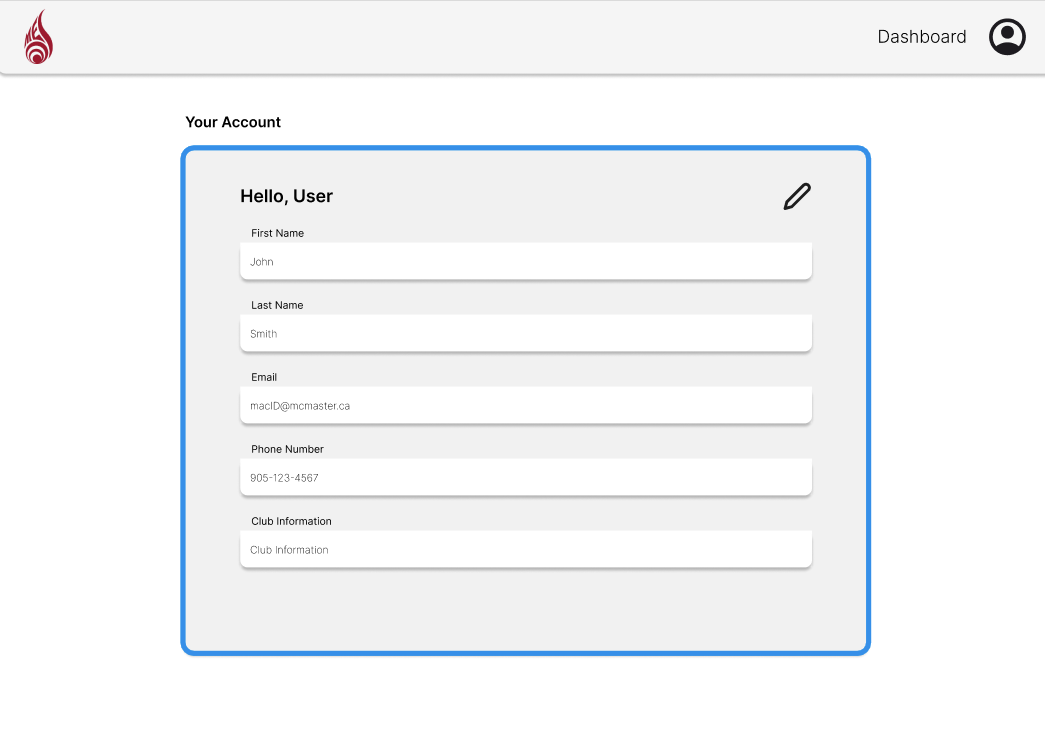
\includegraphics[]{imgs/AccountInfoPage.png}

\subsection{Edit Account Info Page}
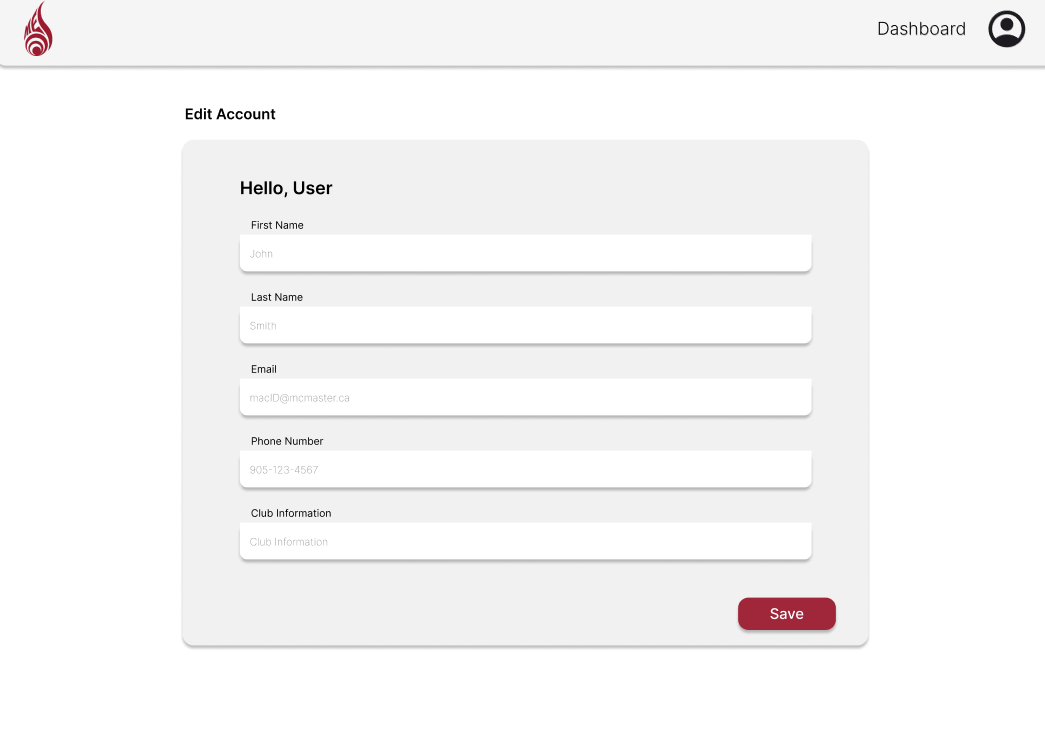
\includegraphics[]{imgs/EditAccountInfoPage.png}

\subsection{Request Page}
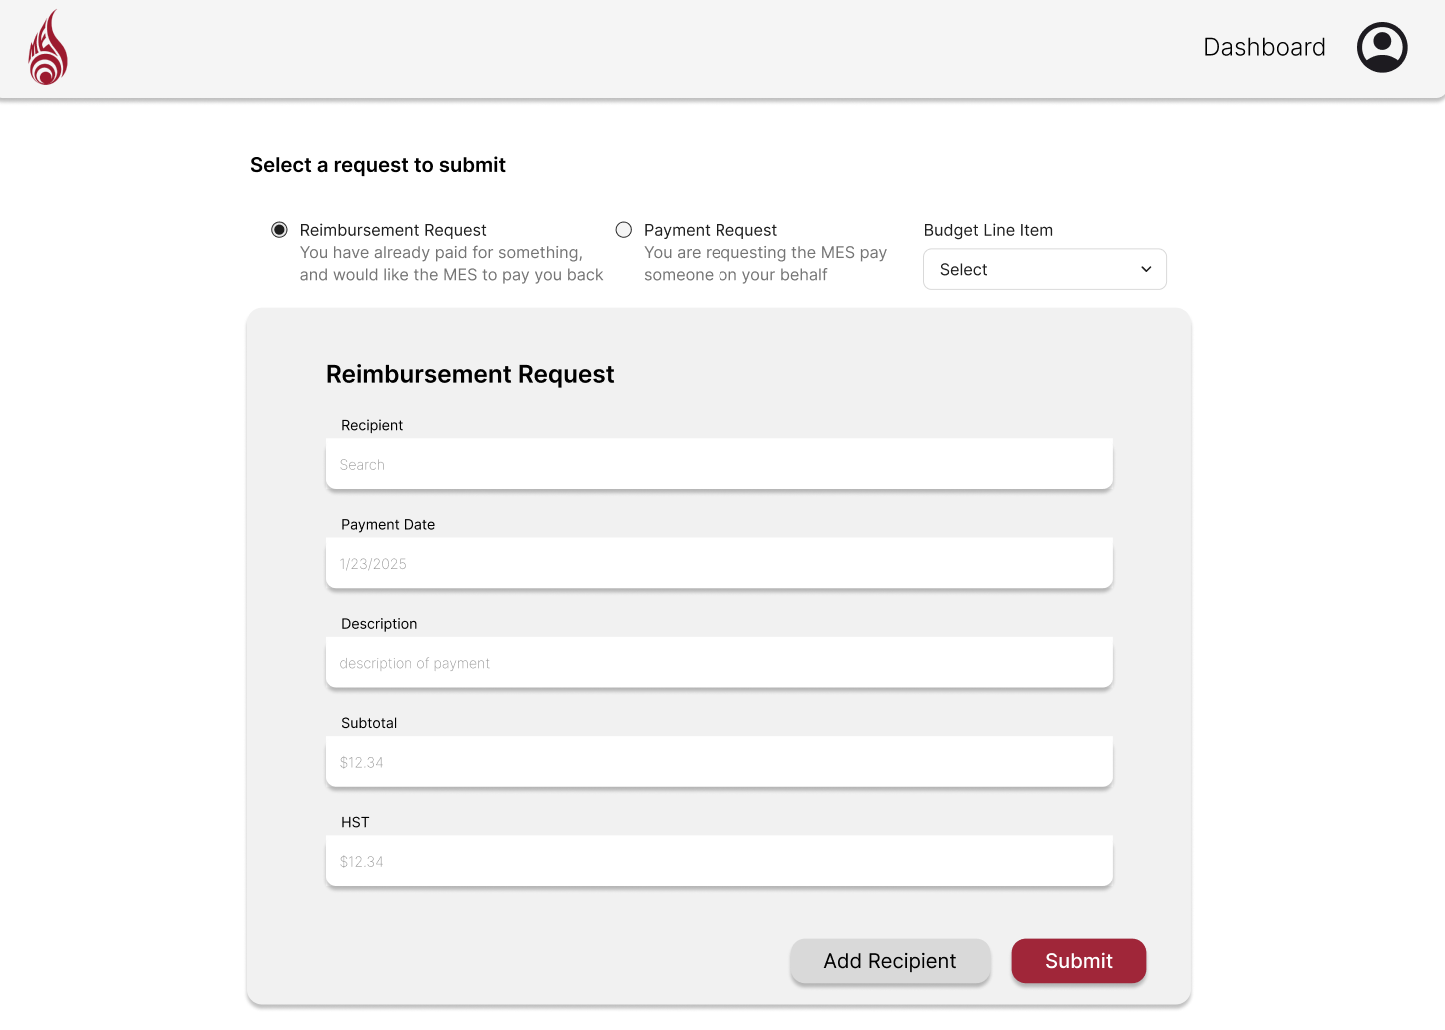
\includegraphics[]{imgs/RequestPage.png}

\subsection{View Requests Page}
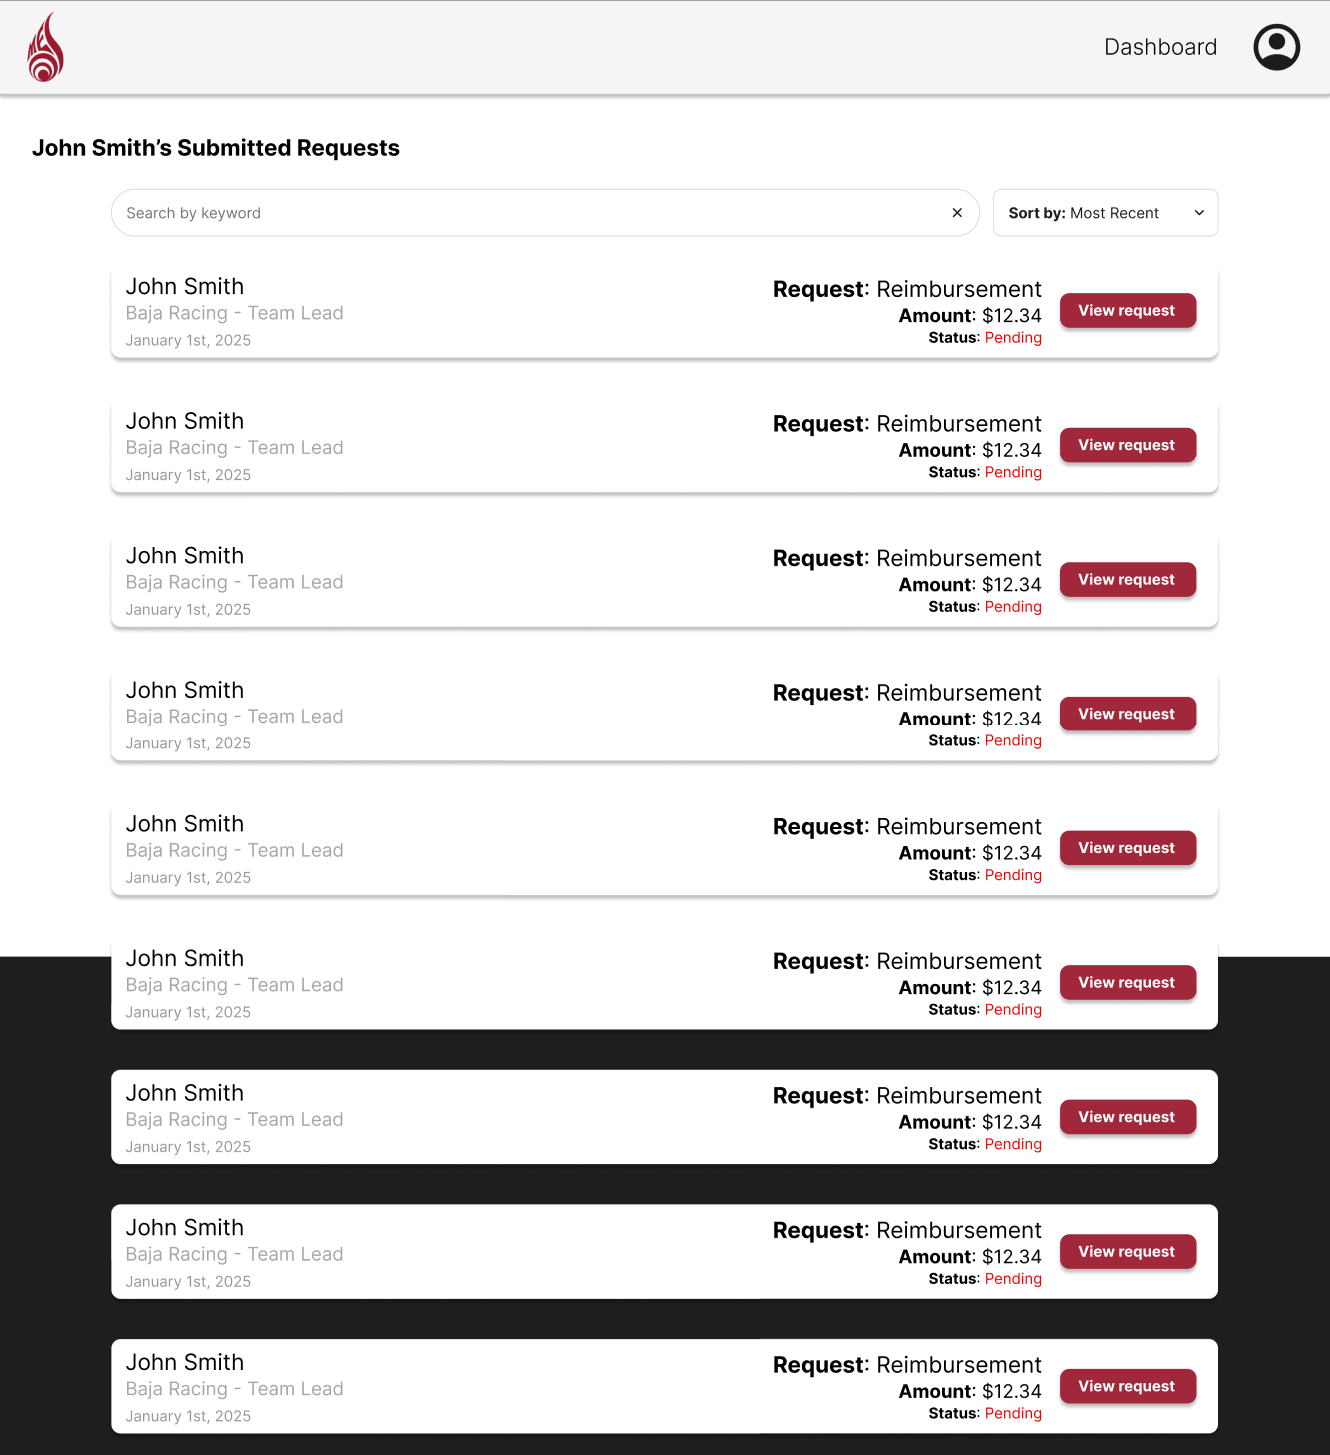
\includegraphics[]{imgs/ViewRequestsPage.png}

\subsection{Edit Request Page (Student/Admins}
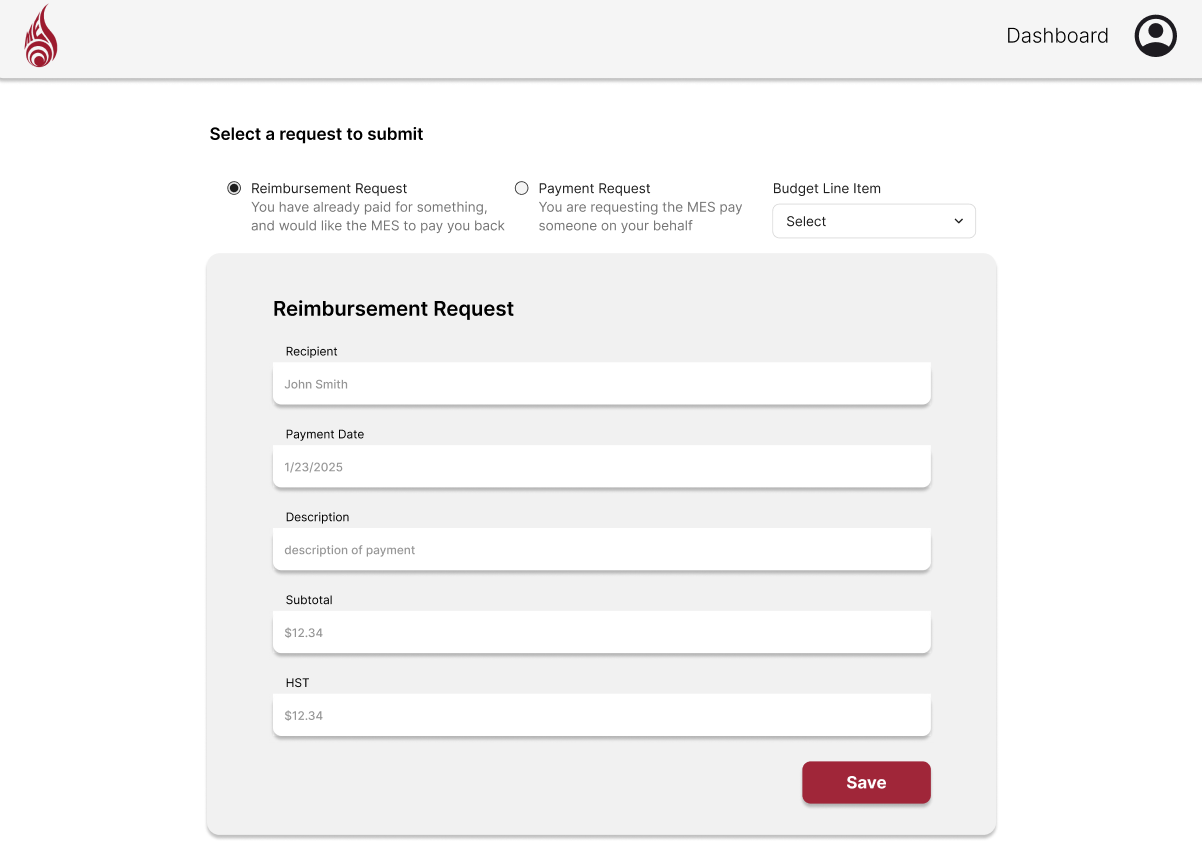
\includegraphics[]{imgs/EditRequestPage.png}

\subsection{Review Request Page (Admins)}
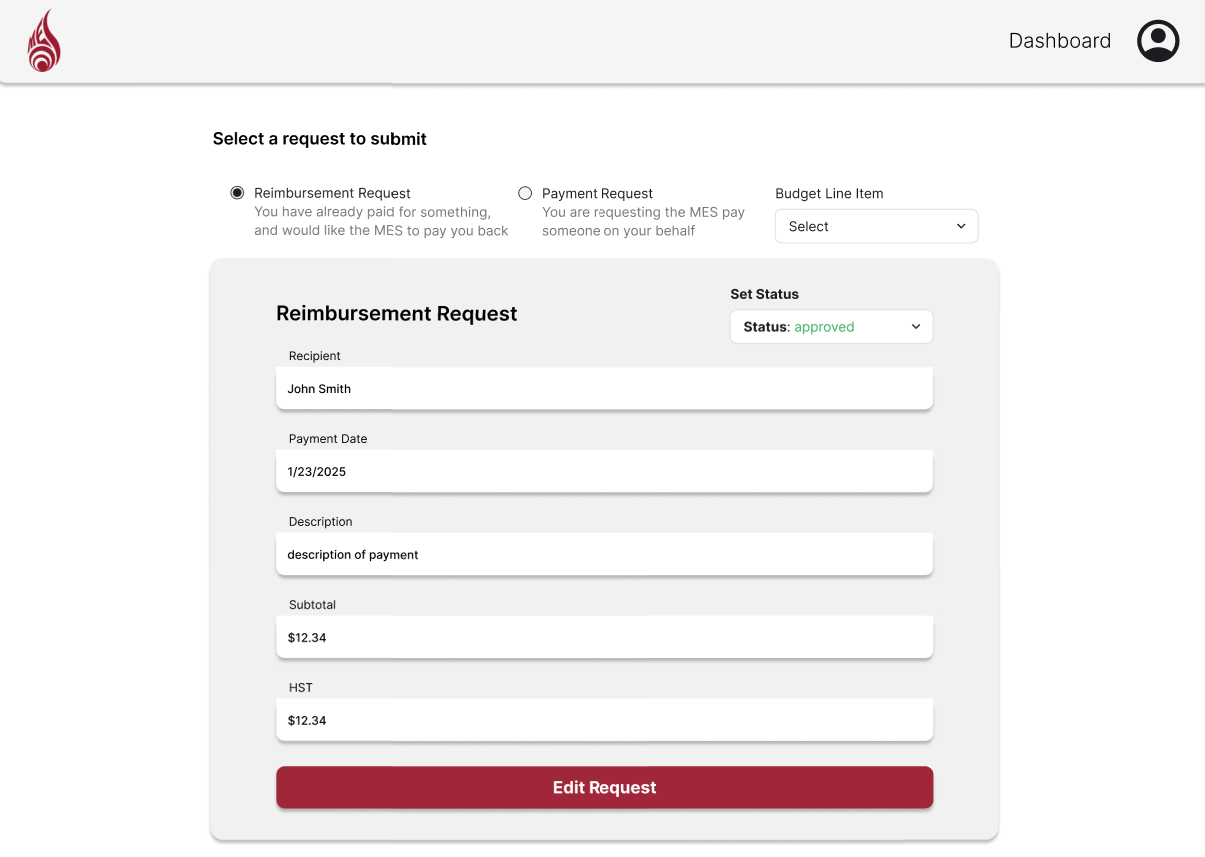
\includegraphics[]{imgs/ReviewRequestAdmins.png}

\subsection{Review Request Page (Students)}
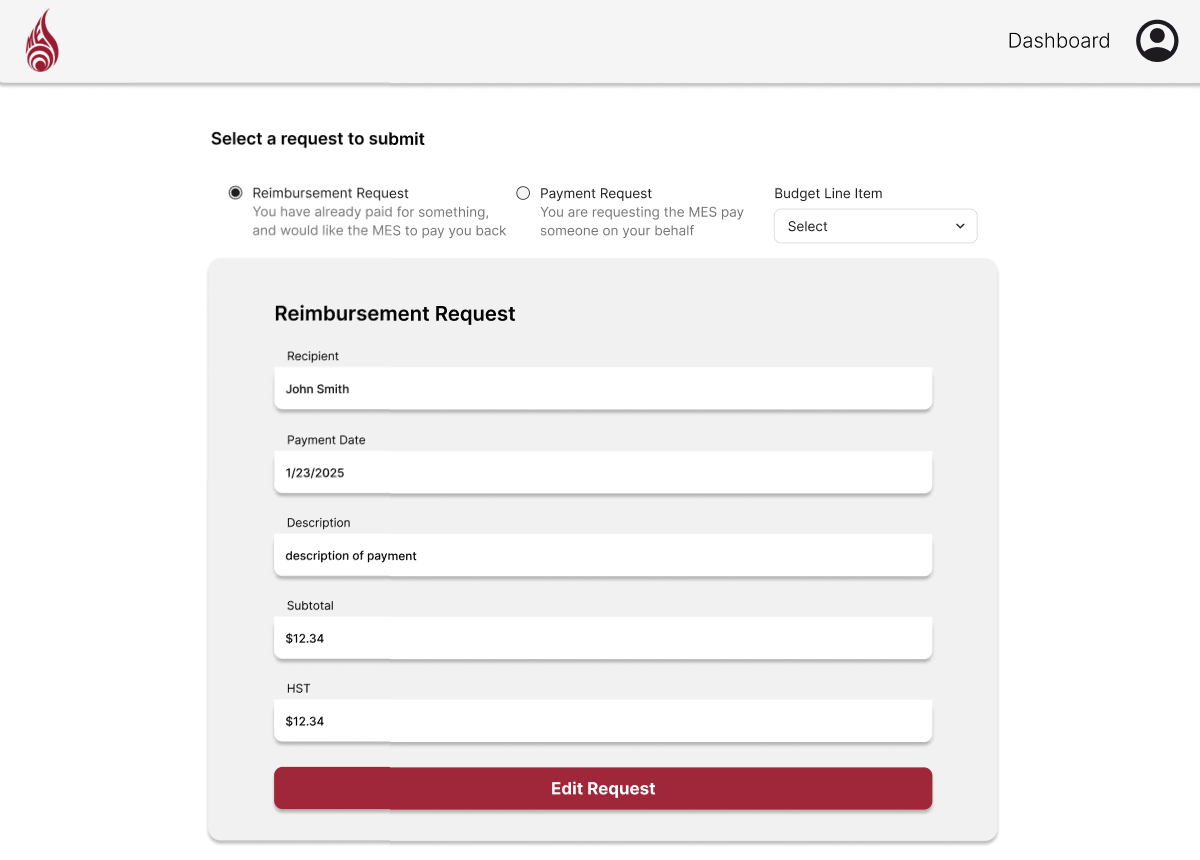
\includegraphics[]{imgs/ReviewRequestStudent.png}

\subsection{Ledger Tracker}
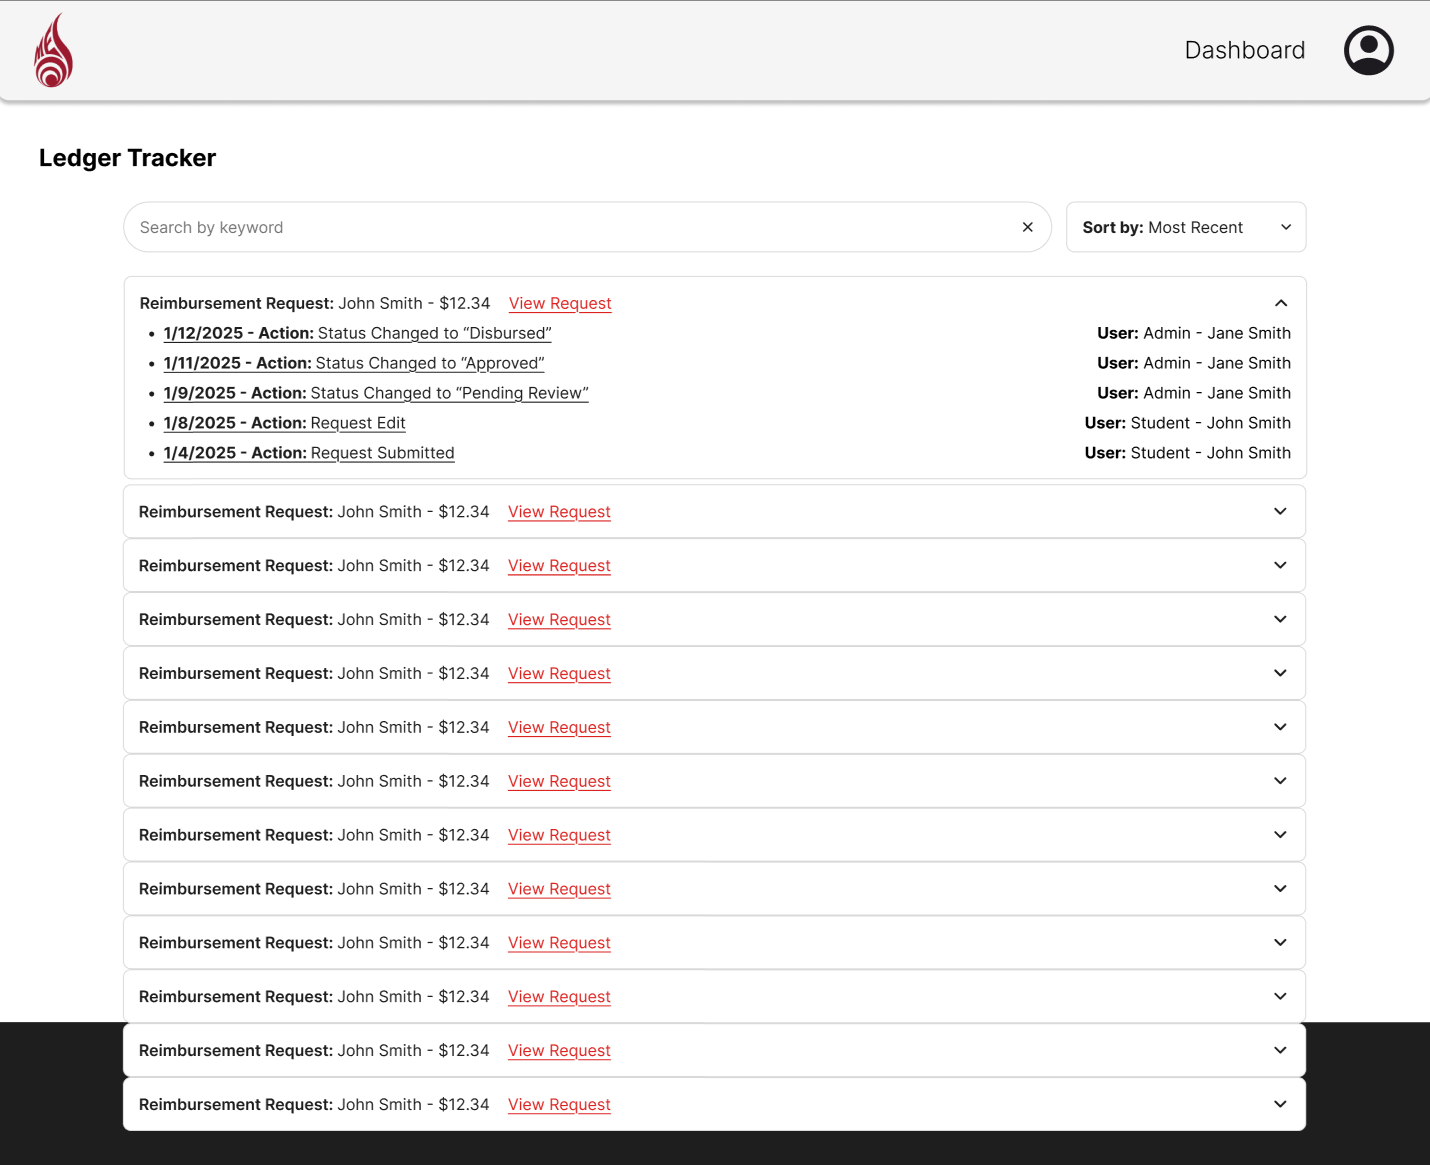
\includegraphics[]{imgs/LedgerTracker.png}

\wss{Design of user interface for software and hardware.  Attach an appendix if
needed. Drawings, Sketches, Figma}

\newpage

\section{Design of Communication Protocols}
Not applicable for this project.

\wss{If appropriate}

\section{Timeline}

Timeline will be found on GitHub Projects \href{https://github.com/users/ausbennett/projects/3/views/6}{here}! 

\wss{Schedule of tasks and who is responsible}

\wss{You can point to GitHub if this information is included there}

%\bibliographystyle {plainnat}
%\bibliography{../../../refs/References}

\newpage{}

\end{document}
